\documentclass[14pt]{beamer}
%\documentclass[handout]{beamer} %Makes Handouts
\usetheme{Singapore} %Gray with fade at top
\useoutertheme[subsection=false]{miniframes} %Supppress subsection in header
\useinnertheme{rectangles} %Itemize/Enumerate boxes
\usecolortheme{seagull} %Color theme
\usecolortheme{rose} %Inner color theme

\definecolor{light-gray}{gray}{0.75}
\definecolor{dark-gray}{gray}{0.55}
\setbeamercolor{item}{fg=light-gray}
\setbeamercolor{enumerate item}{fg=dark-gray}

\setbeamertemplate{navigation symbols}{}
\setbeamertemplate{mini frames}{}
%\setbeamercovered{dynamics}
\setbeamerfont*{title}{size=\Large,series=\bfseries}
\setbeamerfont{footnote}{size=\tiny}

%\setbeameroption{notes on second screen} %Dual-Screen Notes
%\setbeameroption{show only notes} %Notes Output

\setbeamertemplate{frametitle}{\vspace{.5em}\bfseries\insertframetitle}
\newcommand{\heading}[1]{\noindent \textbf{#1}\\ \vspace{1em}}
\newcommand{\questions}{\frame{\vspace{4em}\centering{\Large Questions?}}}
\newcommand{\Ractivity}[1]{\frame{\vspace{4em}\centering{\Large Let's work in R!\\ \vspace{1em} {(#1)}}}}


\usepackage{bbding,color,multirow,times,ccaption,tabularx,graphicx,verbatim,booktabs}
\usepackage{colortbl} %Table overlays
\usepackage[english]{babel}
\usepackage[latin1]{inputenc}
\usepackage[T1]{fontenc}
\usepackage{lmodern}
\usepackage{alltt}

\usepackage{tikz}
\usetikzlibrary{shapes,arrows,decorations.pathreplacing,calc}


\author[]{Thomas J. Leeper}
\institute{
  Government Department\\London School of Economics and Political Science
}


\title{Experimental Research in Legislative Studies}

\date[]{18 August 2017}

\begin{document}

\frame{\titlepage}


\frame{

\frametitle{Activity!}

\only<2-4,6>{
\begin{enumerate}
\item<2-4,6> Ask you to guess a number
\item<3-4,6> Number off 1 and 2 across the room
\item<4,6> Group 2, close your eyes
\item<6> Group 1, close your eyes
\end{enumerate}
}

\Large
\only<5>{\textit{Group 1}\\ Think about whether the population of Chicago is more or less than 500,000 people. What do you think the population of Chicago is?}
\only<7>{\textit{Group 2}\\ Think about whether the population of Chicago is more or less than 10,000,000 people. What do you think the population of Chicago is?}

}
\frame{}

\frame{

\frametitle{Enter your data}

\begin{itemize}\itemsep1em
\item Go here: \url{http://bit.ly/297vEdd}
\item Enter your guess and your group number
\end{itemize}

%http://goo.gl/forms/xDW4FLm9pau0O8zz2

}


\frame{

\frametitle{Results}

\begin{itemize}\itemsep1em
\item True population: 2.79 million
\item<2-> What did you guess? \href{https://docs.google.com/spreadsheets/d/1SKWljS1EeNkAV5V0NZUwrKOu3LQFILVMB37xfTxyrPM/edit?usp=sharing}{(See Responses)}
\item<3-> What's going on here?
	\begin{itemize}
	\item An experiment!
	\item Demonstrates ``anchoring'' heuristic
	\end{itemize}
\item<4-> Experiments are easy to analyze, but only if designed and implemented well
\end{itemize}

}

\frame{\tableofcontents[subsubsectionstyle=hide]}

\frame{
\frametitle{Who am I?}

\small

\begin{itemize}\itemsep0.25em

\item Thomas Leeper

\item Assistant Professor in Political Behaviour at London School of Economics

\begin{itemize}
\item 2013--15: Aarhus University (Denmark)
\item 2008--12: PhD from Northwestern University (Chicago, USA)
\item Birth--2008: Minnesota, USA
\end{itemize}

\item Interested in survey and experimental methods and political psychology

\item Email: \href{mailto:t.leeper@lse.ac.uk}{t.leeper@lse.ac.uk}

\end{itemize}

}


\frame{

\frametitle{Who are you?}

\begin{itemize}\itemsep1em

\item Where are you from?

\item Have you designed a survey and/or experiment before?

\item What do you hope to learn from the course?

\end{itemize}

}



\frame{

\frametitle{Quick Survey}

\begin{enumerate}\itemsep0.5em
\item<2-> How many of you have worked with survey data before?
\item<3-> Of those, how many of you have \textit{performed} a survey before?
\item<4-> How many of you have worked with experimental data before?
\item<5-> Of those, how many of you have \textit{performed} an experiment before?
\end{enumerate}

}


\frame{

\frametitle{Course Materials}

\begin{center}
All material for the course is available at:\\

\vspace{1em}

\url{http://www.thomasleeper.com/legexpcourse/}
\end{center}

}

\frame{

\frametitle{Learning Outcomes}

\small

By the end of the day, you should be able to\dots

\begin{enumerate}
\item<2-> Explain how to analyze experiments quantitatively.
\item<3-> Explain how to design experiments that speak to relevant research questions and theories.
\item<4-> Evaluate the uses and limitations of three common legislative experimental paradigms: survey experiments, field experiments, and simulations.
\item<5-> Identify practical issues that arise in the implementation of experiments and evaluate how to anticipate and respond to them.
\end{enumerate}

}




\section[History/Logic]{History and Logic of Experiments}
\frame{\tableofcontents[currentsection,subsubsectionstyle=hide]}

\frame{

\frametitle{Experiments: Definition}

Oxford English Dictionary defines ``experiment'' as:

\begin{enumerate}
\item A scientific procedure undertaken to make a discovery, test a hypothesis, or demonstrate a known fact
\item A course of action tentatively adopted without being sure of the outcome
\end{enumerate}
}

\frame{

\frametitle{Experiments: History}

\begin{itemize}\itemsep0.75em
\item ``Experiments'' have a very long history

\item Major advances in design and analysis of experiments based on agricultural and later biostatistical research in the 19th century (Fisher, Neyman, Pearson, etc.)

\item First randomized, controlled trial (RCT) by Peirce and Jastrow in 1884

	\begin{itemize}
	\item<2-> First experiment by Gosnell (1924)
	\item<2-> Gerber and Green (2000) first major \textit{field} experiment
	\end{itemize}

\end{itemize}

}


\frame{

\frametitle{Survey-Experiments}

\small

\begin{itemize}
\item Rise of surveys in the behavioral revolution
	\begin{itemize}
	\item Experimentation rare because of paper mode
	\item Limited use of ``split ballots''
	\end{itemize}
\item<2-> 1983: Merrill Shanks and the Berkeley Survey Research Center develop \textbf{CATI}
\item<3-> Mid-1980s: Paul Sniderman \& Tom Piazza performed the first survey experiment\only<3->{\footnote{Sniderman, Paul M., and Thomas Piazza. 1993. \textit{The Scar of Race}. Cambridge, MA: Harvard University Press.}}
	\begin{itemize}\footnotesize
	\item Then: the ``first multi-investigator''
	\item Later: Skip Lupia and Diana Mutz created TESS
	\end{itemize}

\end{itemize}

}






\frame{
	\includegraphics[width=\textwidth]{images/correlation.png}
}


\frame{

\frametitle{Addressing Confounding}

In observational research\dots

\begin{enumerate}\itemsep0.5em
\item<2-> Correlate a ``putative'' cause ($X$) and an outcome ($Y$)
\item<3-> Identify all possible confounds (\textbf{Z})
\item<4-> ``Condition'' on all confounds
	\begin{itemize}
	\item Calculate correlation between $X$ and $Y$ at each combination of levels of \textbf{Z}
	\end{itemize}
\item<5-> Basically: $Y = \beta_0 + \beta_1 X + \beta Z + \epsilon $
\end{enumerate}

}


\begin{frame}
\begin{center}
\begin{tikzpicture}[>=latex',circ/.style={draw, shape=circle, node distance=5cm, line width=1.5pt}]
    \draw (0,0) node[left] (X) {\textcolor<2->{red}{Smoking}};
    \draw[->] (X) -- (5,0) node[right] (Y) {Cancer};
    \draw[->] (-3,3) node[above] (Z) {Sex} -- (X);
    \draw[->] (Z) -- (Y);
    \draw[->] (5,2) node[above] (A) {Environment} -- (Y);
    \draw[->] (4,-3) node[below, text width=3cm, align=center] (E) {Genetic\\Predisposition} -- (Y);
    \draw[->] (-2, -2) node[below, text width=2.5cm, align=center] (W) {Parental\\Smoking} -- (X);
    \draw[->] (W) -- (Y);
    \draw<2->[->, dashed, very thick] (E) -- (X);
\end{tikzpicture}
\end{center}
\end{frame}




\frame{

\frametitle{Experiments are different}

\begin{enumerate}\itemsep0.75em
\item<2-> Draw causal inferences through \textit{design} not \textit{analysis}
\item<3-> Randomization breaks selection bias
\item<4-> We don't need to ``control'' for anything
\item<5-> We see ``causal effects'' in the comparison of experimental groups
\end{enumerate}

}


% Mill's method of difference
\frame{
\frametitle{{\normalsize Mill's Method of Difference}}

\small

If an instance in which the phenomenon under investigation occurs, and an instance in which it does not occur, \textbf<2->{have every circumstance save one in common}, that one occurring only in the former; \textbf<2->{the circumstance in which alone the two instances differ, is the} effect, or \textbf<2->{cause}, or an necessary part of the cause, \textbf<2->{of the phenomenon}.
}



\frame{

\frametitle{Definitions}

\only<2>{\textbf{Unit}: A physical object at a particular point in time}

\only<3>{\textbf{Treatment}: An intervention, whose effect(s) we wish to assess relative to some other (non-)intervention}

\only<4>{
\textbf{Potential outcomes}: The outcome for each unit that we would observe if that unit received each treatment
\begin{itemize}
\item Multiple potential outcomes for each unit, but we only observe one of them
\end{itemize}
}

\only<5>{\textbf{Causal effect}: The comparisons between the unit-level potential outcomes under each intervention}

}




% Individual-level effects versus ATEs


\frame{
	\frametitle{The Experimental Ideal}
	\small
	A randomized experiment, or randomized control trial is:
 		\begin{quote}\small
 			The observation of units after, and possibly before, a randomly assigned intervention in a controlled setting, which tests one or more precise causal expectations
 		\end{quote}
 	This is Holland's ``statistical solution'' to the fundamental problem of causal inference
}

\frame{
\frametitle{The Experimental Ideal}
\begin{itemize}\itemsep0.5em
\item It solves both the temporal ordering and confounding problems of observational causal inference
	\begin{itemize}
   		\item Treatment ($X$) is applied by the researcher before outcome ($Y$)
   		\item Randomization means there are no confounding ($Z$) variables
	\end{itemize}
\item<2-> Thus experiments are a ``gold standard'' of causal inference
\item<3-> Basically: $Y = \beta_0 + \beta_1 X + \epsilon $
\end{itemize}
}


\frame{

\frametitle{Neyman-Rubin Potential Outcomes Framework}

If we are interested in some outcome $Y$, then for every unit $i$, there are numerous ``potential outcomes'' $Y*$ only one of which is visible in a given reality. Comparisons of (partially unobservable) potential outcomes indicate causality.

}

\frame{

\frametitle{Neyman-Rubin Potential Outcomes Framework}

Concisely, we typically discuss two potential outcomes:

\begin{itemize}\small
\item $Y_{0i}$, the \textit{potential} outcome \textit{realized} if $X_i = 0$ (b/c $D_i = 0$, assigned to control)
\item $Y_{1i}$, the \textit{potential} outcome \textit{realized} if $X_i = 1$ (b/c $D_i = 1$, assigned to treatment)
\end{itemize}

}


\frame{

\frametitle{Historical Aside}

\small

\begin{itemize}
\item The history of the potential outcomes framework is contested
\item Most people attribute it to Donald Rubin
\item Paul Holland was the first to link to the philosophical discussions of causality
\item Donald Rubin attributes this to Jerzy Neyman (1923)
\item James Heckman denies all of this and attributes it Andrew Roy (1951)
\end{itemize}
}







% design-based experimental inference
\frame{
	\frametitle{Experimental Inference I}
	\small
	\begin{itemize}\itemsep0.5em
    	\item<1-> Each unit has multiple \textit{potential} outcomes, but we only observe one of them, randomly
    	\item<2-> In this sense, we are sampling potential outcomes from each unit's population of potential outcomes
		\only<2->{
			\begin{center}
			\begin{tabular}{ccccc}
			unit & low & high & \onslide<3->{control} & \onslide<4->{etc.} \\ \midrule
			1 & ? & ? & \onslide<3->{?} & \onslide<4->{\dots} \\
			2 & ? & ? & \onslide<3->{?} & \onslide<4->{\dots} \\
			3 & ? & ? & \onslide<3->{?} & \onslide<4->{\dots} \\
			4 & ? & ? & \onslide<3->{?} & \onslide<4->{\dots} \\ \bottomrule
			\end{tabular}
			\end{center}
		}
	\end{itemize}
}

\frame{
	\frametitle{Experimental Inference II}
	\small
	\begin{itemize}\itemsep0.5em
    	\item<1-> We cannot see individual-level causal effects
    	\item<2-> We can see \textit{average causal effects}
    		\begin{itemize}
        		\item<2-> Ex.: Average difference in cancer between those who do and do not smoke
    		\end{itemize}
    	\item<3-> We want to know: $TE_i = Y_{1i} - Y_{0i}$
	\end{itemize}
}

\frame{
	\frametitle{Experimental Inference III}
	\small
	\begin{itemize}\itemsep0.5em
		\item<1-> We want to know: $TE_i = Y_{1i} - Y_{0i}$ for every $i$ in the population
		\item<2-> We can average: $E[TE_i] = E[Y_{1i} - Y_{0i}] = E[Y_{1i}] - E[Y_{0i}]$
		\item<3-> But we still only see one potential outcome for each unit:\\ \vspace{1em}
    		$ATE_{naive} = E[Y_{1i} | X = 1] - E[Y_{0i} | X = 0]$
    	\item<4-> Is this what we want to know?
	\end{itemize}
}


\frame{
	\frametitle{Experimental Inference IV}
	\small
	\begin{itemize}\itemsep0.5em
	\item What we want and what we have:
		\begin{align}
		ATE & = E[Y_{1i}] - E[Y_{0i}] \\[1em]
		ATE_{naive} & = E[Y_{1i} | X = 1] - E[Y_{0i} | X = 0]
		\end{align}		
	\item<2-> Are the following statements true?\\
  		\begin{itemize}\itemsep0.5em
      		\item<2-> $E[Y_{1i}] = E[Y_{1i} | X = 1]$
      		\item<2-> $E[Y_{0i}] = E[Y_{0i} | X = 0]$
  		\end{itemize}
  	\item<3-> Not in general!
  	\end{itemize}
}

\frame{
	\frametitle{Experimental Inference V}
	\small
	\begin{itemize}\itemsep0.5em
    	\item Only true when both of the following hold:
    	\begin{align}
    	E[Y_{1i}] = E[Y_{1i} | X = 1] = E[Y_{1i} | X = 0]\\
    	E[Y_{0i}] = E[Y_{0i} | X = 1] = E[Y_{0i} | X = 0]
    	\end{align}
    	\item In that case, potential outcomes are \textit{independent} of treatment assignment
		\item If true (e.g., due to randomization of $X$), then:
    	\begin{align*}
    	ATE_{naive} & = E[Y_{1i} | X = 1] - E[Y_{0i} | X = 0] \tag{5}\\
    	& = E[Y_{1i}] - E[Y_{0i}]\\
    	& = ATE
    	\end{align*}
	\end{itemize}
}

\frame{
	\frametitle{Experimental Inference VI}
	
	
	\normalsize
	\begin{itemize}\itemsep0.5em
    	\item This holds in experiments because of a \textit{physical process of randomization}\footnote{Random means ``known probability of treatment'' not ``haphazard''.}
   		\item<2-> Units differ only in side of coin that was up
	   		\begin{itemize}\footnotesize
	   		\item $X_i = 1$ only because $D_i = 1$
	   		\end{itemize}
	   	\item<3-> Implications:
		   	\begin{itemize}
		   	\item Covariate balance
		   	\item Potential outcomes balanced and independent of treatment assignment
		   	\item No confounding (selection bias)
		   	\end{itemize}
	\end{itemize}
}




\begin{frame}
\small 
\begin{center}
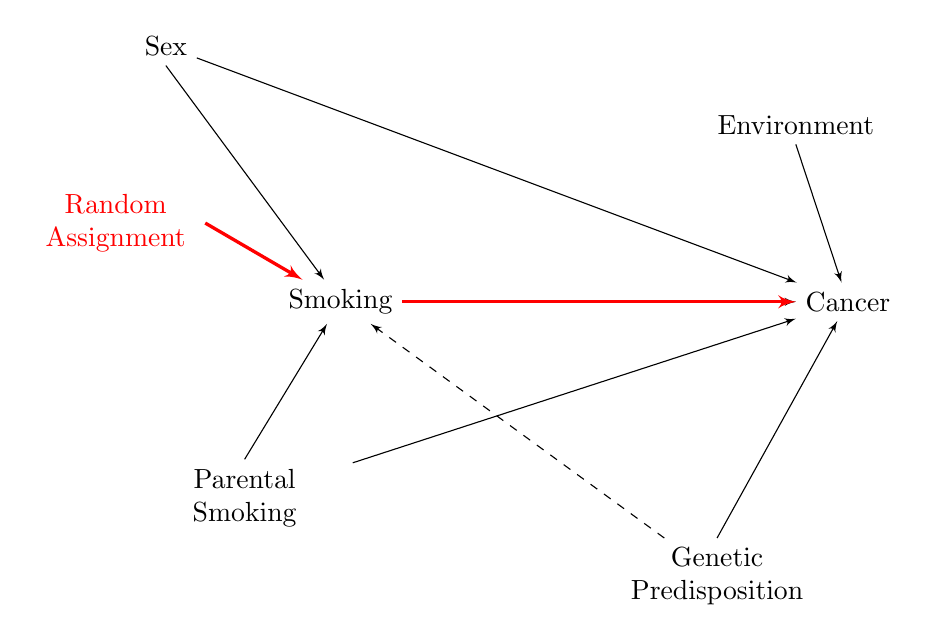
\begin{tikzpicture}[>=latex',circ/.style={draw, shape=circle, node distance=5cm, line width=1.5pt}]
    \draw[->] (0,0) node[left] (X) {Smoking} -- (5,0) node[right] (Y) {Cancer};
    \draw[->] (-3,3) node[above] (Z) {Sex} -- (X);
    \draw[->] (Z) -- (Y);
    \draw[->] (5,2) node[above] (A) {Environment} -- (Y);
    \draw[->] (4,-3) node[below, text width=3cm, align=center] (E) {Genetic\\Predisposition} -- (Y);
    \draw[->] (-2, -2) node[below, text width=2.5cm, align=center] (W) {Parental\\Smoking} -- (X);
    \draw[->] (W) -- (Y);
    \draw[->, dashed] (E) -- (X);
    
    \draw<2->[->, very thick, color=red] (-2.5,1) node[left, color=red, text width=2cm, align=center] (Tr) {Random\\Assignment} -- (X);
    \draw<2->[->, very thick, color=red] (X) -- (Y);
\end{tikzpicture}
\end{center}
\end{frame}



\questions



\frame{
\frametitle{Experimental Analysis I}
\small
\begin{itemize}
\item The statistic of interest in an experiment is the \textit{sample average treatment effect} (SATE)
\item If our sample is \textit{representative}, then this provides an estimate of the population average treatment (PATE)
\item This boils down to being a mean-difference between two groups:
	\begin{equation}
	SATE = \frac{1}{n_1}\sum Y_{1i} - \frac{1}{n_0}\sum Y_{0i}
	\end{equation}
\end{itemize}
}



\frame{

\frametitle{Computation of Effects I}

\begin{itemize}\itemsep0.5em
\item In practice we often estimate SATE using t-tests, ANOVA, or OLS regression
\item These are all basically equivalent
\item<2-> Reasons to choose one procedure over another:
	\begin{itemize}
	\item<2-> Disciplinary norms
	\item<3-> Ease of interpretation
	\item<4-> Flexibility for >2 treatment conditions
	\end{itemize}
\end{itemize}



}

\frame[label=tidy]{

\frametitle{Computation of Effects II}

An experimental data structure looks like:

\small

\begin{center}
\begin{tabular}{ccc}
\texttt{unit} & \texttt{treatment} & \texttt{outcome} \\ \hline 
1 & 0 & 13 \\
2 & 0 & 6 \\
3 & 0 & 4 \\
4 & 0 & 5 \\
5 & 1 & 3 \\
6 & 1 & 1 \\
7 & 1 & 10 \\
8 & 1 & 9 \\ \hline
\end{tabular}
\end{center}

}

\frame{

\frametitle{Computation of Effects II}

Sometimes it looks like this instead, which is bad:

\small

\begin{center}
\begin{tabular}{cccc}
\texttt{unit} & \texttt{treatment} & \texttt{outcome0}  & \texttt{outcome1} \\ \hline 
1 & 0 & 13 & NA \\
2 & 0 & 6 & NA \\
3 & 0 & 4 & NA \\
4 & 0 & 5 & NA \\
5 & 1 & NA & 3 \\
6 & 1 & NA & 1 \\
7 & 1 & NA & 10 \\
8 & 1 & NA & 9 \\ \hline
\end{tabular}
\end{center}

}

\againframe{tidy}



\begin{frame}[fragile]

\frametitle{Computation of Effects III}

R:\small
\begin{verbatim}
t.test(outcome ~ treatment, data = data)
lm(outcome ~ factor(treatment), data = data)
\end{verbatim}

Stata:\small
\begin{verbatim}
ttest outcome, by(treatment)
reg outcome i.treatment
\end{verbatim}

\end{frame}


\questions

\Ractivity{Basic analysis}






\frame{
\frametitle{Experimental Analysis II}
	\small
\begin{itemize}\itemsep0.5em
\item We don't just care about the size of the SATE. We also want to know whether it is significantly different from zero (i.e., different from no effect/difference)
\item To know that, we need to estimate the \textit{variance} of the SATE
\item The variance is influenced by:
	\begin{itemize}
	\item Total sample size
	\item Variance of the outcome, $Y$
	\item Relative size of each treatment group
	\end{itemize}
\end{itemize}
}


\frame{
\frametitle{Experimental Analysis III}
	\small
\begin{itemize}\itemsep0.5em
\item Formula for the variance of the SATE is:\\
$\widehat{Var}(SATE) = \dfrac{\widehat{Var}(Y_0)}{n_0} + \dfrac{\widehat{Var}(Y_1)}{n_1}$

	\begin{itemize}
	\item $\widehat{Var}(Y_0)$ is control group variance
	\item $\widehat{Var}(Y_1)$ is treatment group variance
	\end{itemize}

\item We often express this as the \textit{standard error} of the estimate:\\
$\widehat{SE}_{SATE} = \sqrt{\frac{\widehat{Var}(Y_0)}{n_0} + \frac{\widehat{Var}(Y_1)}{n_1}}$
\end{itemize}
}


\frame{

\frametitle{Intuition about Variance}

\begin{itemize}\itemsep0.5em
\item Bigger sample $\rightarrow$ smaller SEs
\item Smaller variance $\rightarrow$ smaller SEs
\item Efficient use of sample size:
	\begin{itemize}
	\item When treatment group variances equal, equal sample sizes are most efficient
	\item When variances differ, sample units are better allocated to the group with higher variance in \emph{Y}
	\end{itemize}
\end{itemize}


}



\frame{

\frametitle{Statistical Power}

\begin{itemize}\itemsep0.5em
\item Power analysis to determine sample size
\item Type I and Type II Errors
	\begin{itemize}
	\item True positive rate is power
	\item False negative rate is the significance threshold ($\alpha$)
	\end{itemize}
\end{itemize}

\begin{tabular}{lrr}
\toprule
& $H_0$ True & $H_0$ False \\ \midrule
Reject $H_0$ & Type 1 Error & \textbf{True positive} \\
Accept $H_0$ & False negative & Type II error \\ \bottomrule
\end{tabular}

}


\frame{

\frametitle{Doing a Power Analysis}

\begin{itemize}
\item $\mu$, Treatment group mean outcomes
\item $N$, Sample size
\item $\sigma$, Outcome variance
\item $\alpha$ Statistical significance threshold
\item $\phi$, a sampling distribution
\end{itemize}

$Power = \phi\left( \frac{|\mu_1 - \mu_0|\sqrt{N}}{2\sigma} - \phi^{-1}\left( 1 - \frac{\alpha}{2} \right) \right)$

}



\frame{
\frametitle{Intuition about Power}

Minimum detectable effect is the smallest effect we could detect given sample size, ``true'' effect size, variance of outcome, power, and $\alpha$.\\

\vspace{0.5em}

In essence: some non-zero effect sizes are not detectable by a study of a given sample size.\footnote{Gelman, A. and Weakliem, D. 2009. ``Of Beauty, Sex and Power.'' \textit{American Scientist} 97(4): 310--16}

}


\frame{

\frametitle{Intuition about Power}

\begin{itemize}\itemsep0.5em
\item It can help to think in terms of ``standardized effect sizes''
\item Cohen's $d$:\\ $d = \frac{\bar{x}_1 - \bar{x}_0}{s}$, where
$s = \sqrt{\frac{(n_1 - 1)s_1^2 + (n_0 - 1)s_0^2}{n_1 + n_0 - 2}}$
\item Intuition: How large is the effect in standard deviations of the outcome?
	\begin{itemize}
	\item Know if effects are large or small
	\item Compare effects across studies
	\end{itemize}
\item Small: 0.2; Medium: 0.5; Large: 0.8
\end{itemize}

}

\Ractivity{Power Analysis}


\frame{
\frametitle{Intuition about Power}

\begin{center}
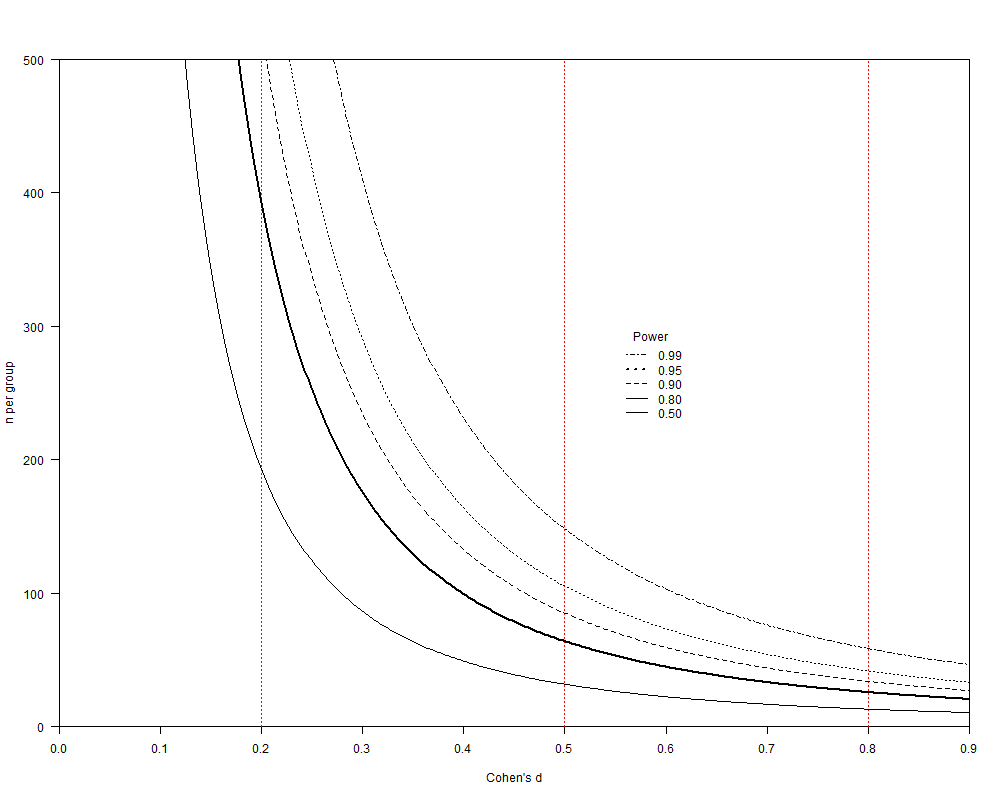
\includegraphics[height=0.8\textheight, trim = 0in 0in 0in 0.5in , clip]{images/power}
\end{center}

}




\frame{}


\section[Theory]{From Theory to Design}
\frame{\tableofcontents[currentsection,subsubsectionstyle=hide]}
% deriving hypotheses from theory and manipulations from hypotheses


\frame{

\frametitle{{\normalsize What kinds of questions can we answer with (survey) experiments?}}

\normalsize

\begin{itemize}\itemsep0.5em
\item<2-> Forward causal questions
	\begin{itemize}
	\item Can X cause Y?
	\item What effects does X have?
	\end{itemize}
\item<3-> Backward causal questions
	\begin{itemize}
	\item What causes Y?
	\item How much of Y is attributable to X?
	\end{itemize}
\item<4-> Even though answering ``forward'' causal question, we start with an outcome concept
\end{itemize}
}



\section[Principles]{Operationalization Principles}

\frame{

\frametitle{Hypothesis Testing}

\begin{itemize}\itemsep0.5em
\item From theory, we derive testable hypotheses
\begin{itemize}
\item Hypotheses are expectations about differences in outcomes across levels of a putatively causal variable
\item Hypothesis must be testable by an SATE
\end{itemize}
\item Manipulations are developed to create variation in that causal variable
\end{itemize}

}


\frame{

\frametitle{{\normalsize Example: News Framing}}

\small

\begin{itemize}
\item Theory: Presentation of news affects opinion
\item Hypotheses:
	\begin{itemize}\footnotesize
	\item News emphasizing free speech increases support for a hate group rally
	\item News emphasizing public safety decreases support for a hate group rally
	\end{itemize}
\item Manipulation:
	\begin{itemize}\footnotesize
	\item Control group: no information
	\item Free speech group: article emphasizing rights
	\item Public safety group: article emphasizing safety
	\end{itemize}
\end{itemize}

}




\frame{

\frametitle{{\normalsize Example: Partisan Identity}}

\small

\begin{itemize}
\item Theory: Strength of partisan identity affects tendency to accept party position
\item Hypotheses:
	\begin{itemize}\small
	\item Strong partisans are more likely to accept their party's position on an issue
	\end{itemize}
\item Manipulation:
	\begin{itemize}\small
	\item Control group: no manipulation
	\item ``Univalent'' condition
	\item ``Ambivalent'' condition
	\end{itemize}
\end{itemize}

}


\frame[label=ambivalentpartisan]{

\frametitle{\textbf{\only<1>{Univalent}\only<2>{Ambivalent}}}

These days, Democrats and Republicans differ from one another considerably. The two groups seem to be growing further and further apart, not only in terms of their opinions but also their lifestyles. Earlier in the survey, you said you tend to identify as a \textit{Democrat/ Republican}. Please take a few minutes to think about what you like about \textit{Democrats/ Republicans} compared to the \textit{Republicans/ Democrats}. Think of 2 to 3 things you especially like best about \textbf{\only<1>{your party}\only<2>{the other party}}. Then think of 2 to 3 things you especially dislike about \textbf{\only<2>{your party}\only<1>{the other party}}. Now please write those thoughts in the space below.

}



\frame{

\frametitle{Treatments Test Hypotheses!}

\begin{itemize}\itemsep0.5em
\item<2-> Derive experimental design from hypotheses
\item<3-> Experimental ``factors'' are expressions of hypotheses as randomized groups
\item<4-> What intervention each group receives depends on hypotheses
	\begin{itemize}
	\item presence/absence
	\item levels/doses
	\item qualitative variations
	\end{itemize}
\end{itemize}

}


\frame{

\frametitle{{\normalsize Ex.: Presence/Absence}}

\small

\begin{itemize}\itemsep0.5em
\item Theory: Negative campaigning reduces support for the party described negatively.
\item Hypothesis: Exposure to a negative advertisement criticizing a party reduces support for that party.
\item Manipulation:
	\begin{itemize}\small 
	\item Control group receives no advertisement. 
	\item Treatment group watches a video containing a negative ad describing a party.
	\end{itemize}
\end{itemize}

}


\frame{

\frametitle{{\normalsize Ex.: Levels/doses}}

\small

\begin{itemize}\itemsep-0.2em
\item Theory: Negative campaigning reduces support for the party described negatively.
\item Hypothesis: Exposure to higher levels of negative advertising criticizing a party reduces support for that party.
\item Manipulation:
	\begin{itemize}\footnotesize
	\item Control group receives no advertisement. 
	\item Treatment group 1 watches a video containing 1 negative ad describing a party.
	\item Treatment group 2 watches a video containing 2 negative ads describing a party.
	\item Treatment group 3 watches a video containing 3 negative ads describing a party.
	\item etc.
	\end{itemize}
\end{itemize}

}


\frame{

\frametitle{{\normalsize Ex.: Qualitative variation}}

\small

\begin{itemize}
\item Theory: Negative campaigning reduces support for the party described negatively.
\item Hypothesis: Exposure to a negative advertisement criticizing a party reduces support for that party, while a positive advertisement has no effect.
\item Manipulation:
	\begin{itemize}\footnotesize
	\item Control group receives no advertisement. 
	\item Negative treatment group watches a video containing a negative ad describing a party.
	\item Positive treatment group watches a video containing a positive ad describing a party.
	\end{itemize}
\end{itemize}

}

\questions


\frame{}



\frame{

\frametitle{Activity!}

\begin{itemize}\itemsep0.5em
\item How do we know if an experiment is any good?
\item Talk with a partner for about 3 minutes
\item Try to develop some criteria that allow you to evaluate ``what makes for a good experiment?'' 
\end{itemize}

}


\frame{

\frametitle{Some possible criteria}

\small

\begin{itemize}\itemsep-0.2em
\item Significant results
\item Face validity
\item Coherent for respondents
\item Non-obvious to respondents
\item Simple
\item Indirect/unobtrusive
\item Validated by prior work
\item Innovative/creative
\item \dots
\end{itemize}

}


\frame{

\begin{quote}\large
The best criterion for evaluating the quality of an experiment is whether it manipulated the intended independent variable and controlled everything else by design.
\end{quote}
\onslide<2->{\small\hspace{5em} --Thomas J. Leeper (18 January 2017)}

}

\frame{

\frametitle{How do we know we manipulated what we think we manipulated?}

\small

\begin{itemize}
\item<2-> Outcomes are affected consistent with theory
\item<3-> Before the study using \textit{pilot testing} (or \emph{pretesting})
\item<4-> During the study, using \emph{manipulation checks}
\item<5-> During the study, using \emph{placebos}
\item<6-> During the study, using \textit{non-equivalent outcomes}
\end{itemize}
}

\frame{

\frametitle{I. Outcomes Affected}

\begin{itemize}\itemsep0.5em
\item Follows a circular logic!
\item Doesn't tell us anything if we hypothesize null effects
\end{itemize}

}


\frame{

\frametitle{II. Pilot Testing}

\small

\begin{itemize}\itemsep0.2em
\item Goal: establish construct validity of manipulation
\item Assess whether a set of possible manipulations affect a measure of the \textit{independent} variable
\item<2-> Example:
	\begin{itemize}
	\item Goal: Manipulate the ``strength'' of an argument
	\item Write several arguments
	\item Ask pilot test respondents to report how strong each one was
	\end{itemize}
\end{itemize}

}

\frame{

\frametitle{III. Manipulation Checks}

\small

\begin{itemize}\itemsep0.2em
\item Manipulation checks are items added post-treatment, post-outcome that assess whether the \textit{independent} variable was affected by treatment
\item We typically talk about manipulations as directly setting the value of $X$, but in practice we are typically manipulating something \textit{that we think} strongly modifies $X$
\item<2-> Example: information manipulations aim to modify knowledge or beliefs, but are necessarily imperfect at doing so
\end{itemize}

}

\frame{

\frametitle{\normalsize Manipulation check example\footnote{Leeper \& Slothuus. n.d. ``Can Citizens Be Framed?'' Available from: \url{http://thomasleeper.com/research.html}.}}

\begin{enumerate}
\item Treatment 1: Supply Information
\item Manipulation check 1: measure beliefs
\item Treatment 2: Prime a set of considerations
\item Outcome: Measure opinion
\item Manipulation check 2: measure dimension salience
\end{enumerate}

}


\frame{

\frametitle{{\normalsize Some Best Practices}}


\begin{itemize}\itemsep0.5em
\item<2-> Manipulation checks should be innocuous
	\begin{itemize}
	\item Shouldn't modify independent variable
	\item Shouldn't modify outcome variable
	\end{itemize}
\item<3-> Generally, measure post-outcome
\item<4-> Measure both what you wanted to manipulate \textit{and} what you didn't want to manipulate
	\begin{itemize}
	\item Most treatments are \textit{compound}!
	\end{itemize}
\end{itemize}

}

\frame{

\frametitle{IV. Placebos}

\begin{itemize}\itemsep0.5em
\item Include an experimental condition that \textit{does not} manipulate the variable of interest (but might affect the outcome)
\item<2-> Example:
	\begin{itemize}
	\item Study whether risk-related arguments about climate change increase support for a climate change policy
	\item Placebo condition: control article with risk-related arguments about non-environmental issue (e.g., terrorism)
	\end{itemize}
\end{itemize}

}

\frame{

\frametitle{V. Non-equivalent outcomes}

\small

\begin{itemize}\itemsep0.5em
\item Measures an outcome that \textit{should not} be affected by independent variable
\item<2-> Example:
	\begin{itemize}
	\item Assess effect of some treatment on attitudes toward group A
	\item Focal outcome: attitudes toward group A
	\item Non-equivalent outcome: attitudes toward group B
	\end{itemize}
\end{itemize}

}


\frame{

\frametitle{{\normalsize Aside: Demand Characteristics}}

\small

\begin{itemize}\itemsep0.5em
\item ``Demand characteristics'' are features of experiments that (unintentionally) imply the purpose of the study and thereby change respondents' behavior (to be consistent with theory)
\item<2-> Implications:
	\begin{itemize}\footnotesize
	\item Design experimental treatments that are non-obvious
	\item Do not disclose the purpose of the study up front\footnote{But, consider the ethics of not doing so (more Friday)}
	\end{itemize}
\end{itemize}

}




\subsection[Examples]{Common Paradigms and Examples}
\frame{\tableofcontents[currentsection,subsubsectionstyle=hide]}


\frame{

\frametitle{Conclusion}

\begin{itemize}\itemsep0.5em
\item Do we want to know SATE, CATE(s), or both?
\item<2-> Decide in advance
	\begin{itemize}
	\item Include in protocol
	\item Design study to estimate CATE(s)
	\end{itemize}
\item<3-> Estimation of unit-related CATEs
	\begin{itemize}
	\item Block randomization
	\item Post-hoc procedures
	\end{itemize}
\end{itemize}

}


\questions


\section[More Designs]{Beyond One-Shot Designs}
\frame{\tableofcontents[currentsubsection,subsubsectionstyle=hide]}

\frame{

\frametitle{{\normalsize Beyond One-shot Designs}}


\begin{itemize}\itemsep0.5em
\item Surveys can be used as a measurement instrument for a field treatment or a manipulation applied in a different survey panel wave
	\begin{enumerate}
	\item Measure effect duration in two-wave panel
	\item Solicit pre-treatment outcome measures in a two-wave panel
	\item Measure effects of field treatment in post-test only design
	\item Randomly encourage field treatment in pre-test and measure effects in post-test
	\end{enumerate}
\item<2-> Problems? Compliance \& nonresponse
\end{itemize}

}

\frame{

\frametitle{{\normalsize I. Effect Duration}}

\begin{itemize}\itemsep0.5em
\item Use a two- (or more-) wave panel to measure duration of effects
	\begin{itemize}
	\item T1: Treatment and outcome measurement
	\item T2+: Outcome measurement
	\end{itemize}
\item Two main concerns
	\begin{itemize}
	\item Attrition
	\item Panel conditioning
	\end{itemize}
\end{itemize}

}

\frame{

\frametitle{{\normalsize II. Within-Subjects Designs}}

\small

\begin{itemize}
\item Estimate treatment effects as a difference-in-differences
\item Instead of using the post-treatment mean-difference in $Y$ to estimate the causal effect, use the difference in pre-post differences for the two groups:
	\begin{align*}
	(\hat{Y}_{0,t+1} - \hat{Y}_{0,t}) - (\hat{Y}_{j,t+1} - \hat{Y}_{j,t})
	\end{align*}
\item<2-> Advantageous because variance for paired samples decreases as correlation between $t_0$ and $t_1$ observations increases
\end{itemize}

}


\frame{
	\begin{center}
	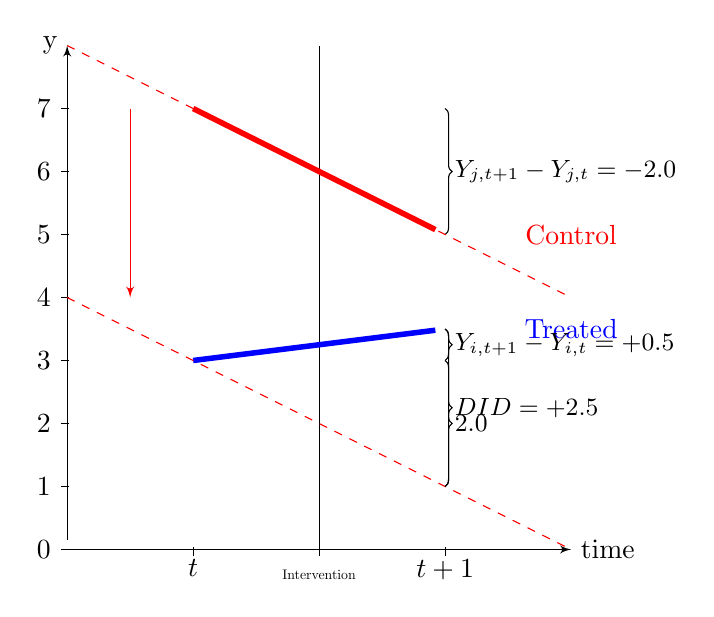
\begin{tikzpicture}[>=latex', scale=0.8]
        \draw[->] (0,0) node (origin) {}  -- (8,0) node[right] (xaxis) {time};
        \draw[->] (origin) -- (0,8) node[left] (yaxis) {y};
        % x ticks
        \foreach \x in {2,4,6}
        	\draw (\x,1pt) -- (\x,-3pt) node[anchor=north] {};
        \draw (2,0) node[below] (before) {$t$};
        \draw (6,0) node[below] (after) {$t+1$};
        \draw (4,-0.25) node[below, scale=0.5] (IV) {Intervention};
        % y ticks
        \foreach \y in {0,...,7}
             \draw (1pt,\y) -- (-3pt,\y) node[anchor=east] {$\y$};
        % intervention
        \draw (4,0) -- (4,8);

        % line
        \draw<2-> (6,3.5) node (tr) {};
        \draw<3-> (6,5) node (ctrl) {};
        \draw<2-3>[blue] (8,3.5) node (trlab) {Treated};
        \draw<3-3>[red] (8,5) node (ctrllab) {Control};        
        \draw<2->[blue, line width=2pt] (2,3) -- (tr);
        \draw<3->[red, line width=2pt] (2,7) -- (ctrl);
        
        % diffs
        \draw<4-6>[right,decorate,decoration={brace,mirror}] 
        	(6,3) -- (6,3.5) node[right, pos=0.5] (idiff) {\small $Y_{i,t+1} - Y_{i,t} = +0.5$};
        \draw<4-6>[right,decorate,decoration={brace}] 
            (6,7) -- (6,5) node[right, pos=0.5] (jdiff) {\small $Y_{j,t+1} - Y_{j,t} = -2.0$};
        
        % trends
        \draw<5-6>[red,->] (1,7) -- (1,4);
        \draw<5->[red, dashed] (0,8) -- (8,4);
        \draw<5->[red, dashed] (0,4) -- (8,0);
        \draw<6>[right,decorate,decoration={brace}] 
            (6,3) -- (6,1) node[right, pos=0.5] (idiff2) {\small $2.0$};
        \draw<7>[right,decorate,decoration={brace}] 
            (6,3.5) -- (6,1) node[right, pos=0.5] (idiff2) {\small $DID = +2.5$};
                        
        
    \end{tikzpicture}
    \end{center}
}


\frame{

	\frametitle{{\normalsize Threats to Validity}}
	
	\small
	
	As soon as time comes into play, we have to worry about threats to validity.\footnote{Shadish, Cook, and Campbell (2002)}
	
	\begin{enumerate}
	\item<2-> History (simultaneous cause)
	\item<3-> Maturation (time trends)
	\item<4-> Testing (observation changes respondents)
	\item<5-> Instrumentation (changing operationalization)
	\item<6-> Instability (measurement error)
	\item<7-> Attrition
	\end{enumerate}
}






\frame{

\frametitle{{\normalsize III. Randomized Field Treatment}}

\small

\begin{itemize}\itemsep-0.2em
\item Examples:
	\begin{enumerate}
	\item<2-> Citizens randomly sent a letter by post encouraging them to reduce water usage
	\item<3-> Different local media markets randomly assigned to receive different advertising
	\end{enumerate}
\item<4-> Survey is used to measure outcomes, when treatment assignment is already known
\item<5-> Issues
	\begin{itemize}
	\item<6-> Nonresponse
	\item<6-> Noncompliance
	\end{itemize}
\end{itemize}

}

\frame{

\frametitle{{\normalsize IV. Treatment Encouragement}}

\small

\begin{itemize}\itemsep-0.2em
\item Design:
	\begin{itemize}
	\item T1: Encourage treatment
	\item T2: Measure effects
	\end{itemize}
\item Examples:
	\begin{enumerate}
	\item Albertson and Lawrence\footnote{Albertson \& Lawrence. 2009. ``After the Credits Roll.'' \textit{American Politics Research} 37(2): 275--300. \href{http://doi.org/10.1177/1532673X08328600}{10.1177/1532673X08328600}.}
	\end{enumerate}
\item<2-> Issues
	\begin{itemize}
	\item<3-> Nonresponse
	\item<3-> Noncompliance
	\end{itemize}
\end{itemize}

}


\frame{

\frametitle{{\normalsize Treatment Noncompliance}}

\begin{itemize}\itemsep0.5em
\item Definition:\\{\small ``when subjects who were assigned to receive the treatment go untreated or when subjects assigned to the control group are treated'' \footnote{Gerber \& Green. 2012. \textit{Field Experiments}, p.132.}}
\item<2-> Several strategies
	\begin{itemize}
	\item ``As treated'' analysis
	\item ``Intention to treat'' analysis
	\item Estimate a LATE
	\end{itemize}
\end{itemize}

}

\frame{
\frametitle{{\normalsize Analyzing Noncompliance}}

\small

\begin{itemize}\itemsep0.5em
\item If noncompliance only occurs in one group, it is \textit{asymmetric} or \textit{one-sided}
\item We can ignore non-compliance and analyze the ``intention to treat'' effect, which will underestimate our effects because some people were not treated as assigned: $ITT = \overline{Y}_1 - \overline{Y}_0$
\item<2-> We can use ``instrumental variables'' to estimate the ``local average treatment effect'' (LATE) for those that complied with treatment: $LATE = \frac{ITT}{\% Compliant}$
\end{itemize}
}

\frame{
	\frametitle{{\large Local Average Treatment Effect}}
	\small
	\begin{itemize}\itemsep0.2em
	\item IV estimate is \textit{local} to the variation in $X$ that is due to variation in $D$
	\item This matters if effects are \textit{heterogeneous}
	\item LATE is effect for those who \textit{comply}
	\item Four subpopulations:
		\begin{itemize}\footnotesize
		\item Compliers: $X = 1$ only if $D = 1$
		\item Always-takers: $X = 1$ regardless of $D$
		\item Never-takers: $X = 0$ regardless of $D$
		\item Defiers: $X = 1$ only if $D = 0$
		\end{itemize}
	\item Exclusion restriction! Monotonicity!
	\end{itemize}
}

\questions






\frame{}

\frame{

\Large

\begin{center}
Quiz time!
\end{center}

}


\frame{
\frametitle{Compliance}

\large

\begin{enumerate}\itemsep0.5em
\item<1-> What is compliance?
\item<2-> How can we analyze experimental data when there is noncompliance?
\end{enumerate}
}

\frame{
\frametitle{Balance testing}

\normalsize

\begin{enumerate}\itemsep0.5em
\item<1-> What does randomization ensure about the composition of treatment groups?
\item<2-> What can we do if we find a covariate imbalance between groups?
\item<3-> How can we avoid this problem entirely?
\end{enumerate}
}


\frame{
\frametitle{Nonresponse and Attrition}

\large

\begin{enumerate}\itemsep0.5em
\item<1-> Do we care about outcome nonresponse in experiments?
\item<2-> How can we analyze experimental data when there is outcome nonresponse or post-treatment attrition?
\end{enumerate}
}


\frame{
\frametitle{Manipulation checks}

\large

\begin{enumerate}\itemsep0.5em
\item<1-> What is a manipulation check? What can we do with it?
\item<2-> What do we do if some respondents ``fail'' a manipulation check?
\end{enumerate}
}



\frame{
\frametitle{Null effects}

\large

\begin{enumerate}\itemsep0.5em
\item<1-> What should we do if we find our estimated $\widehat{SATE} = 0$?
\item<2-> What does it mean for an experiment to be \textit{underpowered}?
\item<3-> What can we do to reduce the probability of obtaining an (unwanted) ``null effect''?
\end{enumerate}
}


\frame{
\frametitle{Effect heterogeneity}

\large

\begin{enumerate}\itemsep0.5em
\item<1-> What should we do if, post-hoc, we find evidence of effect heterogeneity?
\item<2-> What can we do pre-implementation to address possible heterogeneity?
\end{enumerate}
}


\frame{
\frametitle{Representativeness}

\large

\begin{enumerate}\itemsep0.5em
\item<1-> Under what conditions is a design-based, probability sample necessary for experimental inference?
\item<2-> What kind of causal inferences can we draw from an experiment on a descriptively unrepresentative sample?
\end{enumerate}
}

\frame{
\frametitle{Peer Review}

\large

\begin{enumerate}\itemsep0.5em
\item<1-> What should we do if a peer reviewer asks us to ``control'' for covariates in the analysis?
\item<2-> What should we do if a peer reviewer asks us to include or exclude particular respondents from the analysis?
\end{enumerate}
}


\questions





\section{Conclusion}
\frame{\tableofcontents[currentsection,subsubsectionstyle=hide]}




\end{document}
